\chapter[Resultados]{Resultados}

Este capítulo apresenta os resultado obtido com a aplicação dos exemplos de uso descritos no Capítulo XYZ ...

Para melhor organização do trabalho, os resultados serão apresentados em seções, que correspondem à métodos correlacionados.

% palavras chaves para pesquisa
%PROJETO ASEPRITE TABELAS 

\section{Guardas de Inclusão}

As tabelas que contém o detalhamento das execuções dos experimentos se encontram no Apêndice ZYX. A Tabela \ref{tab:resutados_guards_de_inclusao}
sintetiza as médias destes resultados, e a Figura \ref{benchmark_guardas_de_inclusao} apresenta os mesmos dados, em forma
visual. Os tempos são dados em segundos, e os métodos aplicados foram abreviados com as seguintes siglas:

\begin{description}
    \tiny
    \item [GIE:] Guarda de Inclusão Externa
    \item [GII:] Guarda de Inclusão Interna
    \item [PO:]  Pragma Once
    \item [GIIPPO:] Guarda de Inclusão Interna Primeiro que Pragma Once
    \item [POPGII:] Pragma Once Primeiro que Guarda de Inclusão Interna
    \item [GIEPPO:] Guarda de Inclusão Externa e Pragma Once
    \item [RGI:] Redundancia de Guarda de Inclusão
\end{description}

\begin{table}[!ht]
\centering
\caption{Resultados das Guardas de Inclusão}
\label{tab:resutados_guards_de_inclusao}
\begin{tiny}
\begin{tabular}{lp{1cm}p{1cm}p{1cm}p{1cm}p{1cm}p{1cm}p{1cm}p{1cm}}
& \multicolumn{7}{c}{\textbf{Tempo médio de compilação (em segundos)} } \\
\textbf{Sistema Operacional} & \textbf{GIE} & \textbf{GII} & \textbf{PO} &
\textbf{GIIPPO} & \textbf{POPGII} & \textbf{GIEPO} & \textbf{RGI} \\ \toprule
 Linux & 0,2851     & 0,2851  & 1,2127    & 1,3179    & 1,2311  & 1,2477     & 0,1611 \\
 Mac OS Yosemite & 0,8482 & 0,8149 & 1,0031  & 1,0139  & 0,9511  & 0,9097  & 0,5668  \\ 
 Windows 7 & 2,4015 & 2,3954 & 4,2161 & 4,2611 & 4,3152 & 4,2621  & 2,1471 \\
\bottomrule
\end{tabular}
\end{tiny}
\end{table}

\begin{figure}[!h]
    \centering
        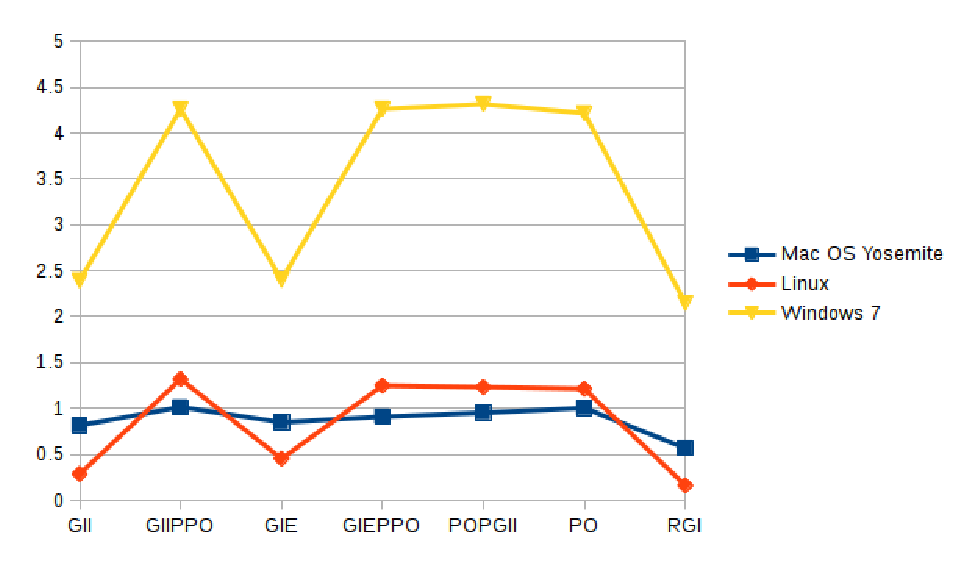
\includegraphics{figuras/graficos/benchmark.eps}
    \caption{Dados coletados dos scripts de Guardas de Inclusão}
    \label{benchmark_guardas_de_inclusao}
\end{figure}

De acordo com dados apresentados, pode-se observe que, para os experimentos em questão, todos os métodos que utilizam a diretiva 
\texttt{\#pragma once} atigiram tempo de compilação superior em relação aos métodos a utilizam, independente do sistema operacional em questão.
Dentre os métodos que não utilizaram esta diretiva, o método \textbf{RGI} foi o que resultou em menor tempo médio de compilação.

Em relação aos sistemas operacionais listados, o Mac OS Yosemite apresentou a menor variação dentre os diferentes métodos, apresentado comportamento 
aproximadamente linear (com média 0,8725 e desvio padrão de 0,1424, o que corresponde a 16\% de variação em torna da média, contra 61\% e 28\% obtido
no Linux e Windows, respectivamente).  No Windows 7, o tempo de compilação dos métodos foi, na maior parte dos métodos, de 3 a 4 vezes maior que nos outros sistemas operacionais. 

\section{Métodos que envolvem a edição do código fonte}

O primeiro método avaliado, que evolve a edição do código fonte, foi a guarda de inclusão \texttt{\#pragma once} (apresentada na Seção XTZ). Este método foi aplicado em todos os 5 projetos selecionado, e os tempos médios de compilação são apresentados na Tabela \ref{tab:pragma}.

\begin{table}[!ht]
\tiny
\centering
\caption{Resultados do \texttt{\#pragma once}}
\label{tab:pragma}
\begin{tabular}{lccccccccc}
& \multicolumn{6}{c}{\textbf{Tempo médio de compilação (em segundos)} } \\
\textbf{Projeto} & \multicolumn{3}{c}{\textbf{Linux}} & \multicolumn{3}{c}{\textbf{Mac OS Yosemite}} & \multicolumn{3}{c}{\textbf{Windows 7}} \\ 
& \textbf{Sem } & \textbf{Com }  & \textbf{Redução (\%)} & \textbf{Sem } & \textbf{Com }  & \textbf{Redução (\%)} & \textbf{Sem } & \textbf{Com }  & \textbf{Redução (\%)} \\
\toprule
Aseprite & 2362 &  2357 & 0,021     & 769  & 772 &   - &  2441 & 2317 & 5,07 \\
iRecoveryplusplus & 1,16 & 0,86     & 25,9 & 2,85 & 2,92 & - & 4,88     & 5,02 & - \\
Pencil & 455  &  459  &  - &  353   & 346  & 1,98 &  530      & 529 &  0,18 \\
Sudoku & 22   &  22   &  - &  38    & 38   & -  &  32 & 29 & 9,37 \\ 
Qcad   & 3923 &  3841 &  2,09  &  3729  & 3290 & 11,77   & - & -  & - \\ 
\end{tabular}
\end{table}

Para os projetos selecionados, o impacto desta técnica não se mostrou relevante, pois em várias configurações não houve sequer ganho em relação ao tempo médio e, nos casos onde
houve ganho, a porcentagem foi muito baixa (exceto no caso do iRecoveryPlus no Linux, com 25\% de ganho, mas o tempo de compilação do projeto já era muito baixo, o que afeta diretamente 
na proporção ganho).

\begin{table}[!ht]
\tiny
\centering
\caption{Resultados da declaração implicita de estrutura}
\label{tab:forward_declaration}
\begin{tabular}{lccccccccc}
& \multicolumn{6}{c}{\textbf{Tempo médio de compilação (em segundos)} } \\
\textbf{Projeto} & \multicolumn{3}{c}{\textbf{Linux}} & \multicolumn{3}{c}{\textbf{Mac OS Yosemite}} & \multicolumn{3}{c}{\textbf{Windows 7}} \\ 
& \textbf{Sem } & \textbf{Com }  & \textbf{Redução (\%)} & \textbf{Sem } & \textbf{Com }  & \textbf{Redução (\%)} & \textbf{Sem } & \textbf{Com }  & \textbf{Redução (\%)} \\
\toprule
iRecoveryplusplus &   1,17  &   0,9  & 23,7 &   2,85 &  2,7 & 5,26 &  4,97 & 4,3 & 13,48 \\
Sudoku   & 22,21  & 20,63   & 7,11  &  38.42  & 36.26  & 5,62 & 32,72 & 27,97 & 14,51  \\ 
\end{tabular}
\end{table}

\begin{table}[!ht]
\tiny
\centering
\caption{Resultados da aplicação ponteiro de implementação privada }
\label{tab:pimpl}
\begin{tabular}{lccccccccc}
& \multicolumn{6}{c}{\textbf{Tempo médio de compilação (em segundos)} } \\
\textbf{Projeto} & \multicolumn{3}{c}{\textbf{Linux}} & \multicolumn{3}{c}{\textbf{Mac OS Yosemite}} & \multicolumn{3}{c}{\textbf{Windows 7}} \\ 
& \textbf{Sem } & \textbf{Com }  & \textbf{Redução (\%)} & \textbf{Sem } & \textbf{Com }  & \textbf{Redução (\%)} & \textbf{Sem } & \textbf{Com }  & \textbf{Redução (\%)} \\
\toprule
iRecoveryplusplus  &   1,17   &  0,91   & 22,22   & 2,85  & 2,70   & 5,26  & 4,97 & 4,83 & 2,81 \\ 
Pencil             &   455    &  454    & 0,22    & 353   & 353    & -     & 530 & 520   & 1,88 \\
Sudoku             &   22,21  & 21,39   & 3,69    & 38,42 & 37,82  & 1,56  & 32,72 & 28,78 & 12,04 \\ 
\end{tabular}
\end{table}

Por fim, os dados detalhados de todos os experimentos com métodos que envolvem a edição do código fonte estão no Apêndice ZRAX.

\section{Métodos que envolvem a parametrização do \textit{build}}


\begin{table}[!ht]
\tiny
\centering
\caption{Resultados parametrização utilizando flags de otimização no Linux}
\label{tab:flags_otimizacao:linux}
\begin{tabular}{lccccccccc}
& \multicolumn{6}{c}{\textbf{Tempo médio de compilação (em segundos)} } \\
 \textbf{Projeto}& \textbf{-O}  & \textbf{-O0}   & \textbf{-O2} & \textbf{-O3} & \textbf{-Os} & \textbf{-Ofast} & \textbf{-Og} & \textbf{Melhor Redução (\%)}\\ \toprule
Aseprite  & 2274 & 2073  & 2357 & 2412 & 2246 & \textbf{705} & 2253 & 70 \\
iRecoveryplusplus   & 1,04 & \textbf{0,89} &  1,17 & 1,12 & 0,90 & 1,13 & 1,03 & 23,93 \\
Pencil  & 456 & 454 &  455 & 455 & \textbf{453} & 455 & 455 & 0,44\\
Sudoku  & 22,23  & 22,51  & 22,21 & 21,92 & \textbf{19,65} & 21,92 & 22,08 &  11,53 \\ 
Qcad    & 3919 &  3925 &  3923 & 3919 & \textbf{3886} & 3922 & 3937 & 0,94  \\ 
\end{tabular}
\end{table}


\begin{table}[!ht]
\tiny
\centering
\caption{Resultados parametrização utilizando flags de otimização no Mac OS Yosemite}
\label{tab:flags_otimizacao:mac_os}
\begin{tabular}{lccccccccc}
& \multicolumn{6}{c}{\textbf{Tempo médio de compilação (em segundos)} } \\
 \textbf{Projeto}& \textbf{-O}  & \textbf{-O0}   & \textbf{-O2} & \textbf{-O3} & \textbf{-Os} & \textbf{-Ofast} & \textbf{Melhor Redução (\%)}\\ \toprule
Aseprite & 775 &  592 &  769 & 795 & 708 & \textbf{209}  & 72,82 \\ 
iRecoveryplusplus & 2,90 & \textbf{2,57} & 2,85 & 2,83 &  2,76  & 2,86  & 9,82 \\ 
Pencil & 353 & \textbf{352} & 353  & 353  & 364 & 356 &  0,39 \\ 
Sudoku & 38,36 & 38,50 & 38,42 & \textbf{38,32} & 39,38 & 38,34 & 0,26  \\ 
Qcad   & 3795 & \textbf{3079} & 3729  & 3737 & 3793  & 3786 &  17,43  \\ 
\end{tabular}
\end{table}

\begin{table}[!ht]
\tiny
\centering
\caption{Resultados parametrização utilizando flags de otimização no Windows 7}
\label{tab:flags_otimizacao:windows}
\begin{tabular}{lccccccccc}
& \multicolumn{6}{c}{\textbf{Tempo médio de compilação (em segundos)} } \\
 \textbf{Projeto}& \textbf{-O}  & \textbf{-O0}   & \textbf{-O2} & \textbf{-O3} & \textbf{-Os} & \textbf{-Ofast} & \textbf{-Og} & \textbf{Melhor Redução (\%)}\\ \toprule
Aseprite &  2254 & 2092 & 2441 & 2550 & 2231 & \textbf{620} & 2184 & 74,6  \\ 
iRecoveryplusplus & 4,58 & 4,65 & 4,97 & 5,17 & \textbf{4,53} & 4,95 &  4,85 &  8,85 \\ 
Pencil & 516 & \textbf{501} & 530  & 534  & 522 & 539 & 513 & 5,47 \\ 
Sudoku & 31,15 & \textbf{29,29} & 32,72 & 35,28 & 31,41 & 35,69 & 30,11 & 16,98 \\ 
\end{tabular}
\end{table}

\section{Alteração de flags de processamento paralelo}

\begin{table}[!ht]
\tiny
\centering
\caption{Resultados parametrização utilizando flags de processamento paralelo no Linux}
\label{tab:flags_processamento_paralelo:linux}
\begin{tabular}{lccccccc}
& \multicolumn{4}{c}{\textbf{Tempo médio de compilação (em segundos)} } \\
\textbf{Projeto} & master & \textbf{-j 2} & \textbf{-j 4} & \textbf{-j 6} & \textbf{-j 8} & \textbf{-j10} &  \textbf{Melhor Redução (\%)} \\ \toprule
Aseprite & 2357 & 1390 & \textbf{1229} & 1479 & 1695 & 1439 & 47,85  \\ 
iRecoveryplusplus & 1,17 & \textbf{1,11} &  1,12 & 1,13 & 1,13 & 1,12 & 5,13 \\ 
Pencil & 455 & 271 & \textbf{242} & 257 & 284 & 288 &  46,81 \\ 
Sudoku & 22 & 13 & 13 & 13 & 14 & \textbf{10} & 54,54  \\ 
Qcad & 3923 & 2437 & \textbf{2301} & 2323 & 1603 & 1557 & 41,34 \\ 
\end{tabular}
\end{table}


\begin{table}[!ht]
\tiny
\centering
\caption{Resultados parametrização utilizando flags de processamento paralelo no Mac OS Yosemite}
\label{tab:flags_processamento_paralelo:mac_os}
\begin{tabular}{lccccccc}
& \multicolumn{4}{c}{\textbf{Tempo médio de compilação (em segundos)} } \\
\textbf{Projeto} &  master & \textbf{-j 2} & \textbf{-j 4} & \textbf{-j 6} & \textbf{-j 8} & \textbf{-j10} &  \textbf{Melhor Redução (\%)} \\ \toprule
Aseprite  & 769 & 576 & 575 & \textbf{288} & 578 & 571 &  62,54 \\ 
iRecoveryplusplus & 2,85 & 2,50 & 2,73 &  2,50 &  2,41 &  \textbf{2,33} & 18,24\\ 
Pencil & 353  & 279 & 275 & 282 & 276 & \textbf{265} & 24,92 \\ 
Sudoku &  38   & 28,27 & 28,17 & 27,97 & 28,31 & \textbf{27,94} & 26,47 \\ 
Qcad   & 3729  & 3596 & 3685 & 3745 & 3422 & \textbf{3103}  & 16,78 \\ 
\end{tabular}
\end{table}

\begin{table}[!ht]
\tiny
\centering
\caption{Resultados parametrização utilizando flags de processamento paralelo no Windows 7}
\label{tab:flags_processamento_paralelo:windows}
\begin{tabular}{lccccccc}
& \multicolumn{4}{c}{\textbf{Tempo médio de compilação (em segundos)} } \\
\textbf{Projeto} & master & \textbf{-j 2} & \textbf{-j 4} & \textbf{-j 6} & \textbf{-j 8} & \textbf{-j10} &  \textbf{Melhor Redução (\%)} \\ \toprule
Aseprite & 2441 & 1140 & 1093 & \textbf{1005} & 1083 & 1022  &  58,82  \\ 
iRecoveryplusplus & 4,97  & 4,99 &  5,02 & 5,11 & 5,01 & \textbf{4,94} & 0,60 \\ 
Pencil & 530 & 262,35 & 259,95 & \textbf{258,90} & 259,15 & 266,47  & 51,15 \\ 
Sudoku & 32,72   & 17,32 & 17,84 & \textbf{16,57} & 18,43 & 18,14 & 49,36 \\ 
\end{tabular}
\end{table}


\section{Métodos que envolvem o uso de ferramentas externas}


\begin{table}[!ht]
\tiny
\centering
\caption{Resultados com uso da ferramenta ccache}
\label{tab:ccache}
\begin{tabular}{lccccccccc}
& \multicolumn{6}{c}{\textbf{Tempo médio de compilação (em segundos)} } \\
\textbf{Projeto} & \multicolumn{3}{c}{\textbf{Linux}} & \multicolumn{3}{c}{\textbf{Mac OS Yosemite}} & \multicolumn{3}{c}{\textbf{Windows 7}} \\ 
& \textbf{Sem } & \textbf{Com }  & \textbf{Redução (\%)} & \textbf{Sem } & \textbf{Com }  & \textbf{Redução (\%)} & \textbf{Sem } & \textbf{Com }  & \textbf{Redução (\%)} \\
\toprule
Aseprite & 2357,87 & 540,58 & 77,07 & 769,16 & 209,82 & 72,72  & 2441,38 & 761,73  & 68,80 \\ 
iRecoveryplusplus & 1,17 & 1,14 & 2,56    & 2,85 & 2,63 & 7,71  & 4,97 & 5,04 & -  \\ 
Pencil & 455  & 173 & 61,98 & 353 & 104  & 70,54  & 530  & 181  & 65,85 \\ 
Sudoku & 22 & 4 & 81,81  & 38 & 7 & 81,58  & 32 & 8  &  75    \\ 
Qcad  & 3923 & 1823 & 53,53 & 3729 & 664 & 82,19 &  -  & -  & -  \\ 
\end{tabular}
\end{table}

\begin{table}[!ht]
\tiny
\centering
\caption{Resultados com uso da ferramenta gold}
\label{tab:gold}
\begin{tabular}{lccc}
& \multicolumn{3}{c}{\textbf{Tempo médio de compilação (em segundos)} } \\
\textbf{Projeto} & \multicolumn{3}{c}{\textbf{Linux}} \\ 
& \textbf{Sem } & \textbf{Com }  & \textbf{Redução (\%)} \\
\toprule
Aseprite & 2357 & 2270  & 3,69 \\
iRecoveryplusplus & 1,17 & 1,00 & 14,52 \\
Pencil & 455  & 457,37 & - \\ 
Sudoku & 22 & 21,17 & 3,77  \\
Qcad  & 3923 & 3847 & 1,94 \\
\end{tabular}
\end{table}
